\documentclass[a4paper,12pt,russian]{article} %draft
\usepackage[T2A]{fontenc}% Поддержка русских букв


% XeTeX packages
\usepackage[cm-default]{fontspec} % or install lmodern and remove cm-default opt
\usepackage{xunicode} % some extra unicode support
\usepackage{xltxtra} % \XeLaTeX macro


\tolerance=1000
\emergencystretch=0.74cm
\usepackage{indentfirst} %делать отступ в начале параграфа

\usepackage[pdfborder = {0 0 0}]{hyperref} %гиперссылки в документе.

\usepackage[utf8]{inputenc}	% кодировка текста
\usepackage[russian]{babel}	% руссификация по Бабелю
\usepackage{graphics}

\usepackage[clean,pdf]{svg}

\usepackage{amsmath, amsfonts} % для расширенных настроек ссылок на формулы
\usepackage{extsizes}	% использование шрифтов большего кегля 

\usepackage{fancyvrb} % Добавляет продвинутые Verbatim и Verb

\usepackage{epsfig} % удобно вставлять рисунки в строку текста
\usepackage[usenames,dvipsnames]{pstricks}
\usepackage{pst-grad} % For gradients
\usepackage{pst-plot} % For axes

\usepackage{graphicx,xcolor}

%\usepackage[MakeStamp]{eskdi}
%\usepackage[MakeStamp, SubSectInToc]{eskdi}
%\usepackage[MakeStamp, SubSubSectInToc]{eskdi}
%\usepackage[MakeStamp, ParagraphInToc]{eskdi}
%\usepackage[twoside, MakeStamp, ParagraphInToc]{eskdi}
%\usepackage{eskdi}
%\usepackage[SubSectInToc]{eskdi}
%\usepackage[SubSubSectInToc]{eskdi}
%\usepackage[ParagraphInToc]{eskdi}
%\usepackage[ParagraphInToc, NumIntoSections]{eskdi}
%\usepackage[twoside, ParagraphInToc]{eskdi}
%\usepackage[twoside, MakeEmptyStamp, ParagraphInToc]{eskdi}
\usepackage[twoside, MakeEmptyStamp]{eskdi}
%\usepackage[MakeEmptyStamp, ParagraphInToc]{eskdi}



\usepackage{array}
\usepackage{tabularx}
\usepackage{supertabular}
\usepackage{longtable} % для создания таблиц, переносящихся на другую страницу
%\usepackage{listingsutf8}%
\usepackage{listings} % для включения листинга кода в приложения. Русский язык глючит.


\lstloadlanguages{bash,[LaTeX]TeX,MetaPost,Clean,Matlab}


\usepackage{textcomp}	% Ввод различных знаков
\usepackage{keystroke} % для отображения символов клавиш
\usepackage{bytefield} %для создания таблиц с битовыми полями
\usepackage{filecontents} %для включения в документ содержимого файлов

\usepackage{tikz} % Пакет для рмсования диаграмм
\usepackage{tikz-timing}[2009/12/09]
\usetikzlibrary{positioning,arrows,automata,plotmarks} %В данном случае нам потребуются positioning и arrows, которые нужны для расположения элементов друг относительно друга и рисования стрелок между ними соответственно.
\usetikzlibrary{shapes,snakes}
\usepackage{schemabloc}

\usepackage{makecell} % Для многострочных ячеек таблицы
\usepackage{colortbl} % Для раскрашивания ячеек в таблицах


%{Arial} {Courier New} 
%{OpenGost Type A TT} {OpenGost Type B TT} % Свободный шрифт. Нет наклонного начертания и дирного начертания
%{GOST type A} % Морально устарел, не свободный, не хватает символа тирэ. Не рекомендуется
%{GOST type B} % Морально устарел, не свободный, не хватает символа тирэ. Не рекомендуется
\gostSetRomanfont{Times New Roman}%
\gostSetSansfont{Times New Roman}%
\gostSetMonofont{Times New Roman}%
\gostSetMainfont{Times New Roman}%
\gostSetStampfont{Arial}%


%\verbatimfont{\fontspec[Scale=1.0]{Arial} \itshape}% % Для замены стиля начертания verbatim и verb
\verbatimfont{\fontspec[Scale=1.0]{Consolas}}% % Для замены стиля начертания verbatim и verb
\newfontfamily{\gostListingfont}[Scale=1.0]{Consolas} % Шрифт для листингов
%\renewcommand{\SetStampfontIt}{\itshape}%

%\input commands.tex %Файл включает такие команды как надчёркивание, запрещение переноса ТУ и др.
\setpage % Разметка текста на странице
\begin{document}

	\gosttitleobject{Лабораторная работа}
		
	\gosttitledocument{ПОСТРОЕНИЕ И ИССЛЕДОВАНИЕ МОДЕЛЕЙ ВНЕШНИХ ВОЗДЕЙСТВИЙ
}

	% Раскомментировать если необходима утверждающая надпись на титульном листе
	\renewcommand\titleBotRIGHT{
	\spboxmm{100}{70}{70}{30}{lc}{\parbox{70mm}{
			\normalsize{Преподаватель: Чепинский С.А. }\\ 
			\normalsize{Студенты: Французов Р.А.\\  Донцова М.А.}\\
			\normalsize{Группа: R3325}\\
			\normalsize{Вариант: 18}}}}

		\maketitle
		
		\section{Цель работы}
		Ознакомление с принципами построения моделей внешних воздействий — сигналов задания и возмущений. 
 \\
		
		\section{Ход работы}
Ниже представлены исходные данные варианта\\
\begin{center}
\begin{tabular}{|c|c|}
	\hline
	$\varphi$ & 4
 \\ \hline
	$f$ & 10
 \\ \hline
	$F$ & \input{F} \\ \hline
	$V$ & 2
 \\ \hline
	$\Delta$ & 2
 \\ \hline
	Вид возмущения & $g(t)=4\sin t+3\cos 4t$
 \\ \hline
\end{tabular}
\end{center}


\subsection{Генератор гармонического сигнала}
По исходным данным варианта вычислены амплитуда и угловая частота гармонического сигнала:\\
$\omega=2\pi f=25.13
$\\
$A=\dfrac{180\varphi}{\pi}=229.2
$\\
Опираясь на уравнения 3.2 методических указаний\\
$\dot{z_1}=z_2, \dot{z_2}=-\omega^2z_1, g=z_1, z_2(0)=\omega A$\\
построенна следующая схема моделирования:\\

\begin{figure}[H]
	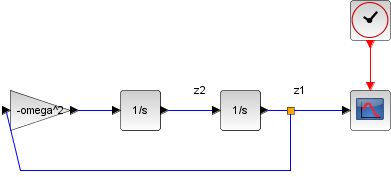
\includegraphics[width=0.5\textwidth]{signal_generator}
	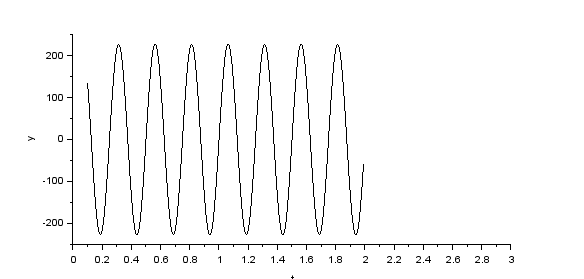
\includegraphics[width=0.7\textwidth]{signal_generator-plot}
	\caption{Схема и результаты моделирования гармонического генератора}
\end{figure}

\subsection{Генератор сигнала с трапецеидальным графиком скорости}
Основываясь на том, что к моменту времени $t_A$ под действием ускорения $\Delta$ скорость должна стать равной $V$ расчитано $t_A=t_{BC}=\dfrac{V}{\Delta}=1$, при этом доказательство равенства отрезков времени не приводится. Найти отрезок времени $t_{AB}$ не представляется возможным, потому как на нем не действует ускорение, а вся продолжительность сигнала не задана; длительность отрезка была принята как 3\\
Модель генератора была составлена и запущена:\\
\begin{figure}[H]
	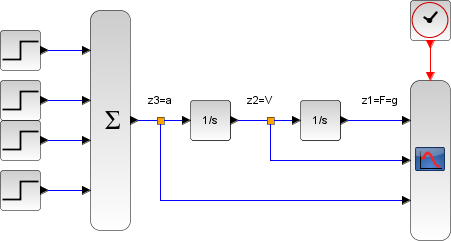
\includegraphics[width=0.5\textwidth]{trapec}
	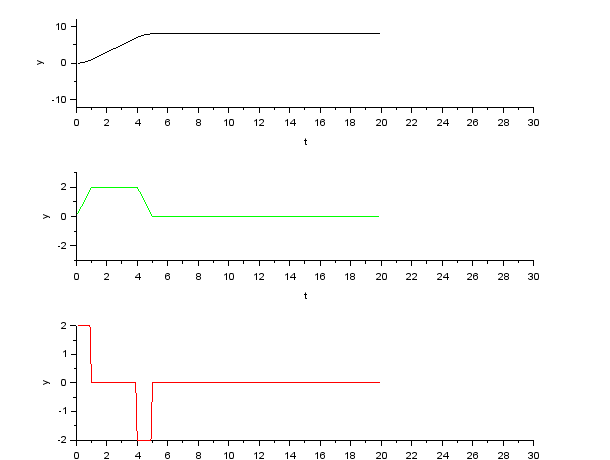
\includegraphics[width=0.7\textwidth]{trapec-plot}
	\caption{Схема и результаты моделирования генератор с трапецеидальным графиком скорости }
\end{figure}

\subsection{Генератор возмущения}
Начальная функция была разбита как сумма двух\\
$g_1=4\sin t\\\dot{g_1}=4\cos t\\ \ddot{g_1}=-4sin t=-g_1\\ \dot{g_1}(0)=4$
 \\

$g_2=3\cos 4t\\\dot{g_2}=-12\sin 4t\\ \ddot{g_2}=-48cos 4t=-16g_2\\ g_2(0)=3$
 \\ 


Были созданны модели обоих генераторов и суммарный сигнал выведен на график:\\
\begin{figure}[H]
	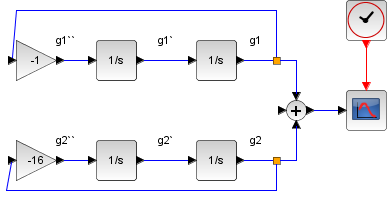
\includegraphics[width=0.5\textwidth]{distortion}
	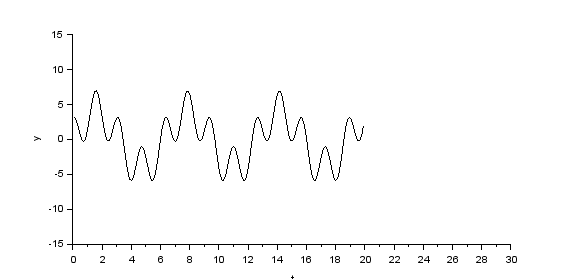
\includegraphics[width=0.7\textwidth]{distortion-plot}
	\caption{Схема и результаты моделирования генератора возмущения}
\end{figure}


\section{Вывод}
В ходе данной работы были успешно составлены и промоделированы генераторы гармонического сигнала, с трапецеидальным графиком скорости и возмущения, состоящего из нескольких гармонических
\end{document}